
% case name
\chapter{waq3d aed2}
%
% - Purpose & Description:
%     These first two parts give reader short details about the test case,
%     the physical phenomena involved, the geometry and specify how the numerical solution will be validated
%
\section{Purpose}
%
This test shows the coupling between \telemac{3d} and the water quality library AED2.
%
\section{Description}
%
A perfectly still basin is considered (length 1m, width 1m, and constant water depth 5m).


%\subsection{Reference}
%
%[1] BARR D. Densimetric exchange flow in rectangular channels.
%III. Large scale experiments. La Houille Blanche, 22, 619-632. 1967.
%
%[2] BENJAMIN T. Gravity currents and related phenomena.
%Journal of Fluid Mechanics, 31(2), 209-248. 1968.
%
%[3] TURNER J. Buoyancy effects in fluids. Cambridge University Press.
%1973.
%
%[4] YIH C.S. Stratified flows. Academic Press. 1980.
%
% - Geometry and Mesh:
%     This part describes the mesh used in the computation
%
%
\subsection{Geometry and Mesh}
%
See Figure \ref{fig:mesh}

\begin{figure} [H]
\centering
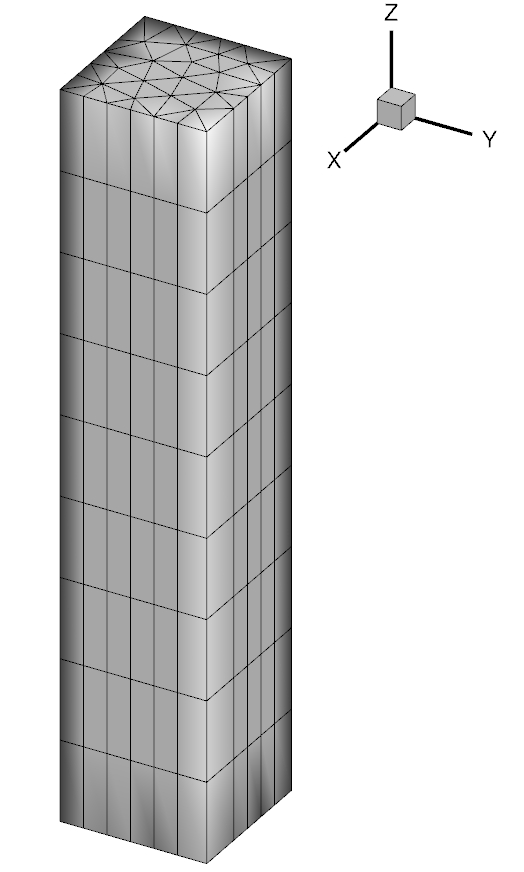
\includegraphics[scale=0.4]{mesh_waq3d-aed2.jpg}
 \caption{waq3d aed2 test: horizontal and vertical meshes}
 \label{fig:mesh}
\end{figure}
%
\subsubsection{Bathymetry}
%
Flat bottom ($z$ = 0~m)
%
\subsubsection{Geometry}
%
Basin length = 1~m\\
Basin width = 1~m
%
\subsubsection{Mesh}
%
36 triangular elements\\
29 nodes\\
10 planes regularly spaced
%
%
% - Physical parameters:
%     This part specifies the physical parameters
%
%
\subsection{Physical parameters}
%
Diffusion: no\\
Coriolis: no\\
Wind: no
%
% Experimental results (if needed)
%\subsection{Experimental results}
%
% bibliography can be here or at the end
%\subsection{Reference}
%
% Section for computational options
%\section{Computational options}
%
% - Initial and boundary conditions:
%     This part details both initial and boundary conditions used to simulate the case
%
\subsection{Water quality parameters}
Coupling with Waqtel and Water quality processes = 6 (AED2)
aed2.nml file contains the AED2 parametrization. The following modules are activated :
\begin{itemize}
	\item sedflux
	\item oxygen
	\item carbon
	\item silica
	\item nitrogen
	\item phosphorus
	\item organic matter
	\item phytoplankton
	\item tracer
	\item total
\end{itemize}
%
\subsection{Initial and Boundary Conditions}
%
\subsubsection{Initial conditions}
%
Constant water depth = 5~m\\
No velocity\\
Initial concentrations are homogeneous
%
\subsubsection{Boundary conditions}
%
Closed boundaries\\
Bottom friction : Strickler law with coefficient 40m$^{1/3}$s$^{-1}$
%
\subsection{General parameters}
%
Time step: 1~s\\
Simulation duration: 1000~s
%
% - Numerical parameters:
%     This part is used to specify the numerical parameters used
%     (adaptive time step, mass-lumping when necessary...)
%
%
\subsection{Numerical parameters}
%
Non-hydrostatic versions\\
%

%
\subsection{Comments}
Among the tracers, only the temperature, the oxygen, methan, silica and phytoplankton concentrations are printed in the result files.

% - Results:
%     We comment in this part the numerical results against the reference ones,
%     giving understanding keys and making assumptions when necessary.
%
%
\section{Results}

As an example the Figure \ref{fig:res} shows the phytoplankton concentration at the end of the calculation.
%

\begin{figure} [H]
\centering
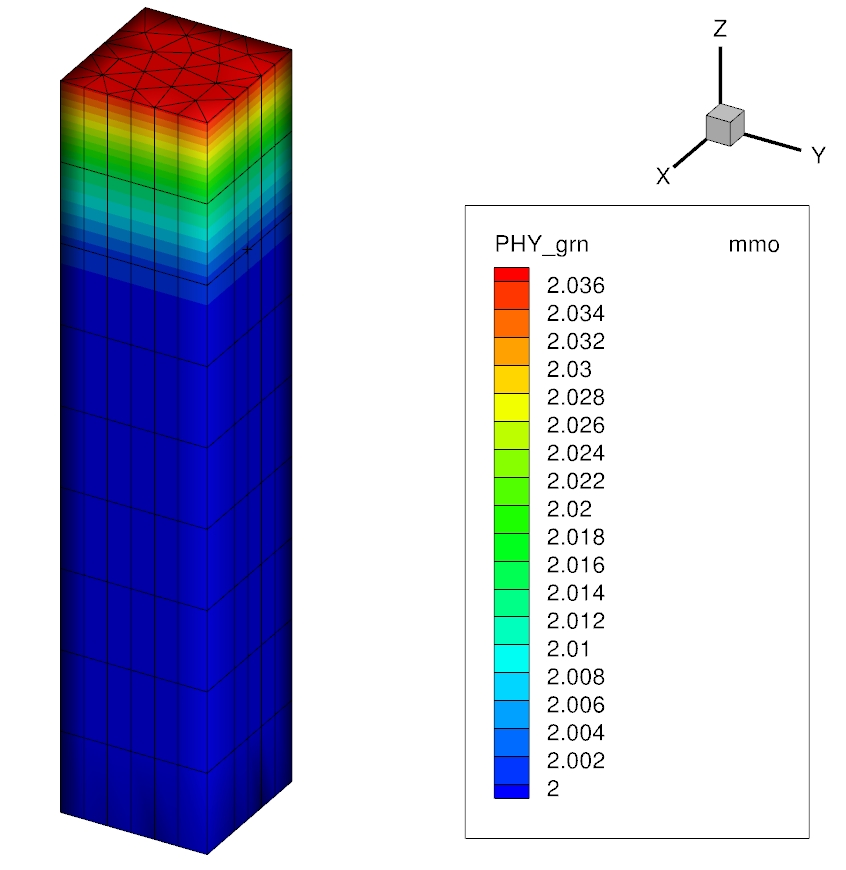
\includegraphics[scale=0.4]{phyto.jpg}
 \caption{waq3d aed2 test: phytoplankton concentration after 1000s.}
 \label{fig:res}
\end{figure}


%
\section{Conclusion}
%
\telemac{3d} is coupled with AED2
%
% Here is an example of how to include the graph generated by validateTELEMAC.py
% They should be in test_case/img
%\begin{figure} [!h]
%\centering
%\includegraphics[scale=0.3]{../img/mygraph.png}
% \caption{mycaption}\label{mylabel}
%\end{figure}
%
% bibliography
%\section{Reference}

